% load TENOR file template

% hfmt-drawsocket
% -----------------------------------------------
% Template for SMAC SMC 2013
% adapted and corrected from the template for SMC 2012, which was adapted from that of SMC 2011
% further updated for TENOR 2015, 2016, 2017 and 2018
% -----------------------------------------------
\documentclass{article}
\usepackage{tenor2019}
\usepackage{ifpdf}
\usepackage[english]{babel}
\usepackage{balance}
\usepackage{listings}
\usepackage{float}

%%%%%%%%%%%%%%%%%%%%%%%% Some useful packages %%%%%%%%%%%%%%%%%%%%%%%%%%%%%%%
%%%%%%%%%%%%%%%%%%%%%%%% See related documentation %%%%%%%%%%%%%%%%%%%%%%%%%%
%\usepackage{amsmath} % popular packages from Am. Math. Soc. Please use the 
%\usepackage{amssymb} % related math environments (split, subequation, cases,
%\usepackage{amsfonts}% multline, etc.)
%\usepackage{bm}      % Bold Math package, defines the command \bf{}
%\usepackage{paralist}% extended list environments
%%subfig.sty is the modern replacement for subfigure.sty. However, subfig.sty 
%%requires and automatically loads caption.sty which overrides class handling 
%%of captions. To prevent this problem, preload caption.sty with caption=false 
%\usepackage[caption=false]{caption}
%\usepackage[font=footnotesize]{subfig}



% paper title, authors
\def\papertitle{drawsocket: A browser based system for networked score display%:  and the St. Pauli Elbtunnel project
}

\def\Hochschule {Hochschule f\"ur Musik und Theater}

\def\firstauthor{Rama Gottfried}
\def\secondauthor{Georg Hajdu}


\title{\papertitle}
 \twoauthors
   {\firstauthor} {	
      Hochschule f\"ur Musik und Theater\\
        Hamburg, Germany \\ %
   \small{\tt \href{mailto:rama.gottfried@hfmt-hamburg.de}{rama.gottfried@hfmt-hamburg.de}}}
    {\secondauthor} {
   Hochschule f\"ur Musik und Theater\\
   Hamburg, Germany \\ %
   \small{\tt \href{mailto:georg.hajdu@hfmt-hamburg.de}{georg.hajdu@hfmt-hamburg.de}}}


 
% other setup


%user defined variables


%\hyphenpenalty10000

\usepackage{xspace}
\def\symbolist{\textsc{symbolist}\xspace}
\def\drawsocket{\textsc{drawsocket}\xspace}
\def\maxscore{\textsc{maxscore}\xspace}
\def\innovativ{Innovative Hochschule: \textit{Stage\textunderscore2.0}\xspace}

\def\oscfontsize{\footnotesize}

\def\oscformat{
  mathescape,
  columns=fullflexible,
  basicstyle=\oscfontsize\fontfamily{lmvtt}\selectfont 
}

\makeatletter
\newcommand{\verbatimfont}[1]{\renewcommand{\verbatim@font}{\ttfamily#1}}
\makeatother


% adds the automatic
% Saves a lot of ouptut space in PDF... after conversion with the distiller
% Delete if you cannot get PS fonts working on your system.

% pdf-tex settings: detect automatically if run by latex or pdflatex
\newif\ifpdf
\ifx\pdfoutput\relax
\else
   \ifcase\pdfoutput
      \pdffalse
   \else
      \pdftrue
\fi

\ifpdf % compiling with pdflatex
  \usepackage[pdftex,
    pdftitle={\papertitle},
    pdfauthor={\firstauthor, \secondauthor},
    bookmarksnumbered, % use section numbers with bookmarks
    pdfstartview=XYZ % start with zoom=100% instead of full screen; 
                     % especially useful if working with a big screen :-)
   ]{hyperref}
  %\pdfcompresslevel=9

  \usepackage[pdftex]{graphicx}
  % declare the path(s) where your graphic files are and their extensions so 
  %you won't have to specify these with every instance of \includegraphics
  \graphicspath{{./figures/}}
  \DeclareGraphicsExtensions{.pdf,.jpeg,.png}

  \usepackage[figure,table]{hypcap}

\else % compiling with latex
  \usepackage[dvips,
    bookmarksnumbered, % use section numbers with bookmarks
    pdfstartview=XYZ % start with zoom=100% instead of full screen
  ]{hyperref}  % hyperrefs are active in the pdf file after conversion

  \usepackage[dvips]{epsfig,graphicx}
  % declare the path(s) where your graphic files are and their extensions so 
  %you won't have to specify these with every instance of \includegraphics
  \graphicspath{{./figures/}}
  \DeclareGraphicsExtensions{.eps}

  \usepackage[figure,table]{hypcap}
\fi

%setup the hyperref package - make the links black without a surrounding frame
\hypersetup{
    colorlinks,%
    citecolor=black,%
    filecolor=black,%
    linkcolor=black,%
    urlcolor=black
}



% ------ Start of Document -----

\begin{document}
%

\capstartfalse
\maketitle
\capstarttrue
%
\begin{abstract}
We present \drawsocket, a new platform for generating synchronized, browser-based displays across an array of networked devices developed at the \Hochschule, Hamburg. 
Conceived as a system for distributed notation display with applications in music and spatial performance contexts, \drawsocket provides a unified interface for controlling diverse media features of web-browsers which can be utilized in many ways.
By providing access to browser mouse and multitouch gesture data, and the ability to dynamically create user-defined callback methods, the \drawsocket system aims to provide a flexible tool for creating graphical user interfaces.
Included is a discussion of the architecture design and development process, followed by an overview of the features, and syntax considerations for the \drawsocket API.

\end{abstract}

\section{drawsocket}\label{sec:drawsocket}
The \drawsocket design approach is based on the ``o.io'' paradigm developed at the University of California, Berkeley's Center for New Music and Technology (CNMAT), which uses the OpenSoundControl (OSC) encoding~\cite{wright:osc} to create a uniform user application programing interface(API) by ``wrapping'' vendor- and protocol-specific details in an interoperable API syntax~\cite{freed2014io, maccallum2015dynamic}.
In this way, the \drawsocket system is an ``o.io'' wrapper for web browser display and interaction, aiming to provide a homogenous OSC API for manipulating the graphic building blocks of Scalable Vector Graphics (SVG),\footnote{https://www.w3.org/TR/SVG11/} Cascading Style Sheets (CSS),\footnote{https://www.w3.org/Style/CSS/specs.en.html} HyperText Markup Language (HTML),\footnote{https://www.w3.org/TR/html52/} and a curated collection of client-based JavaScript libraries for animation and sound production.

\begin{figure*}[]
\centering
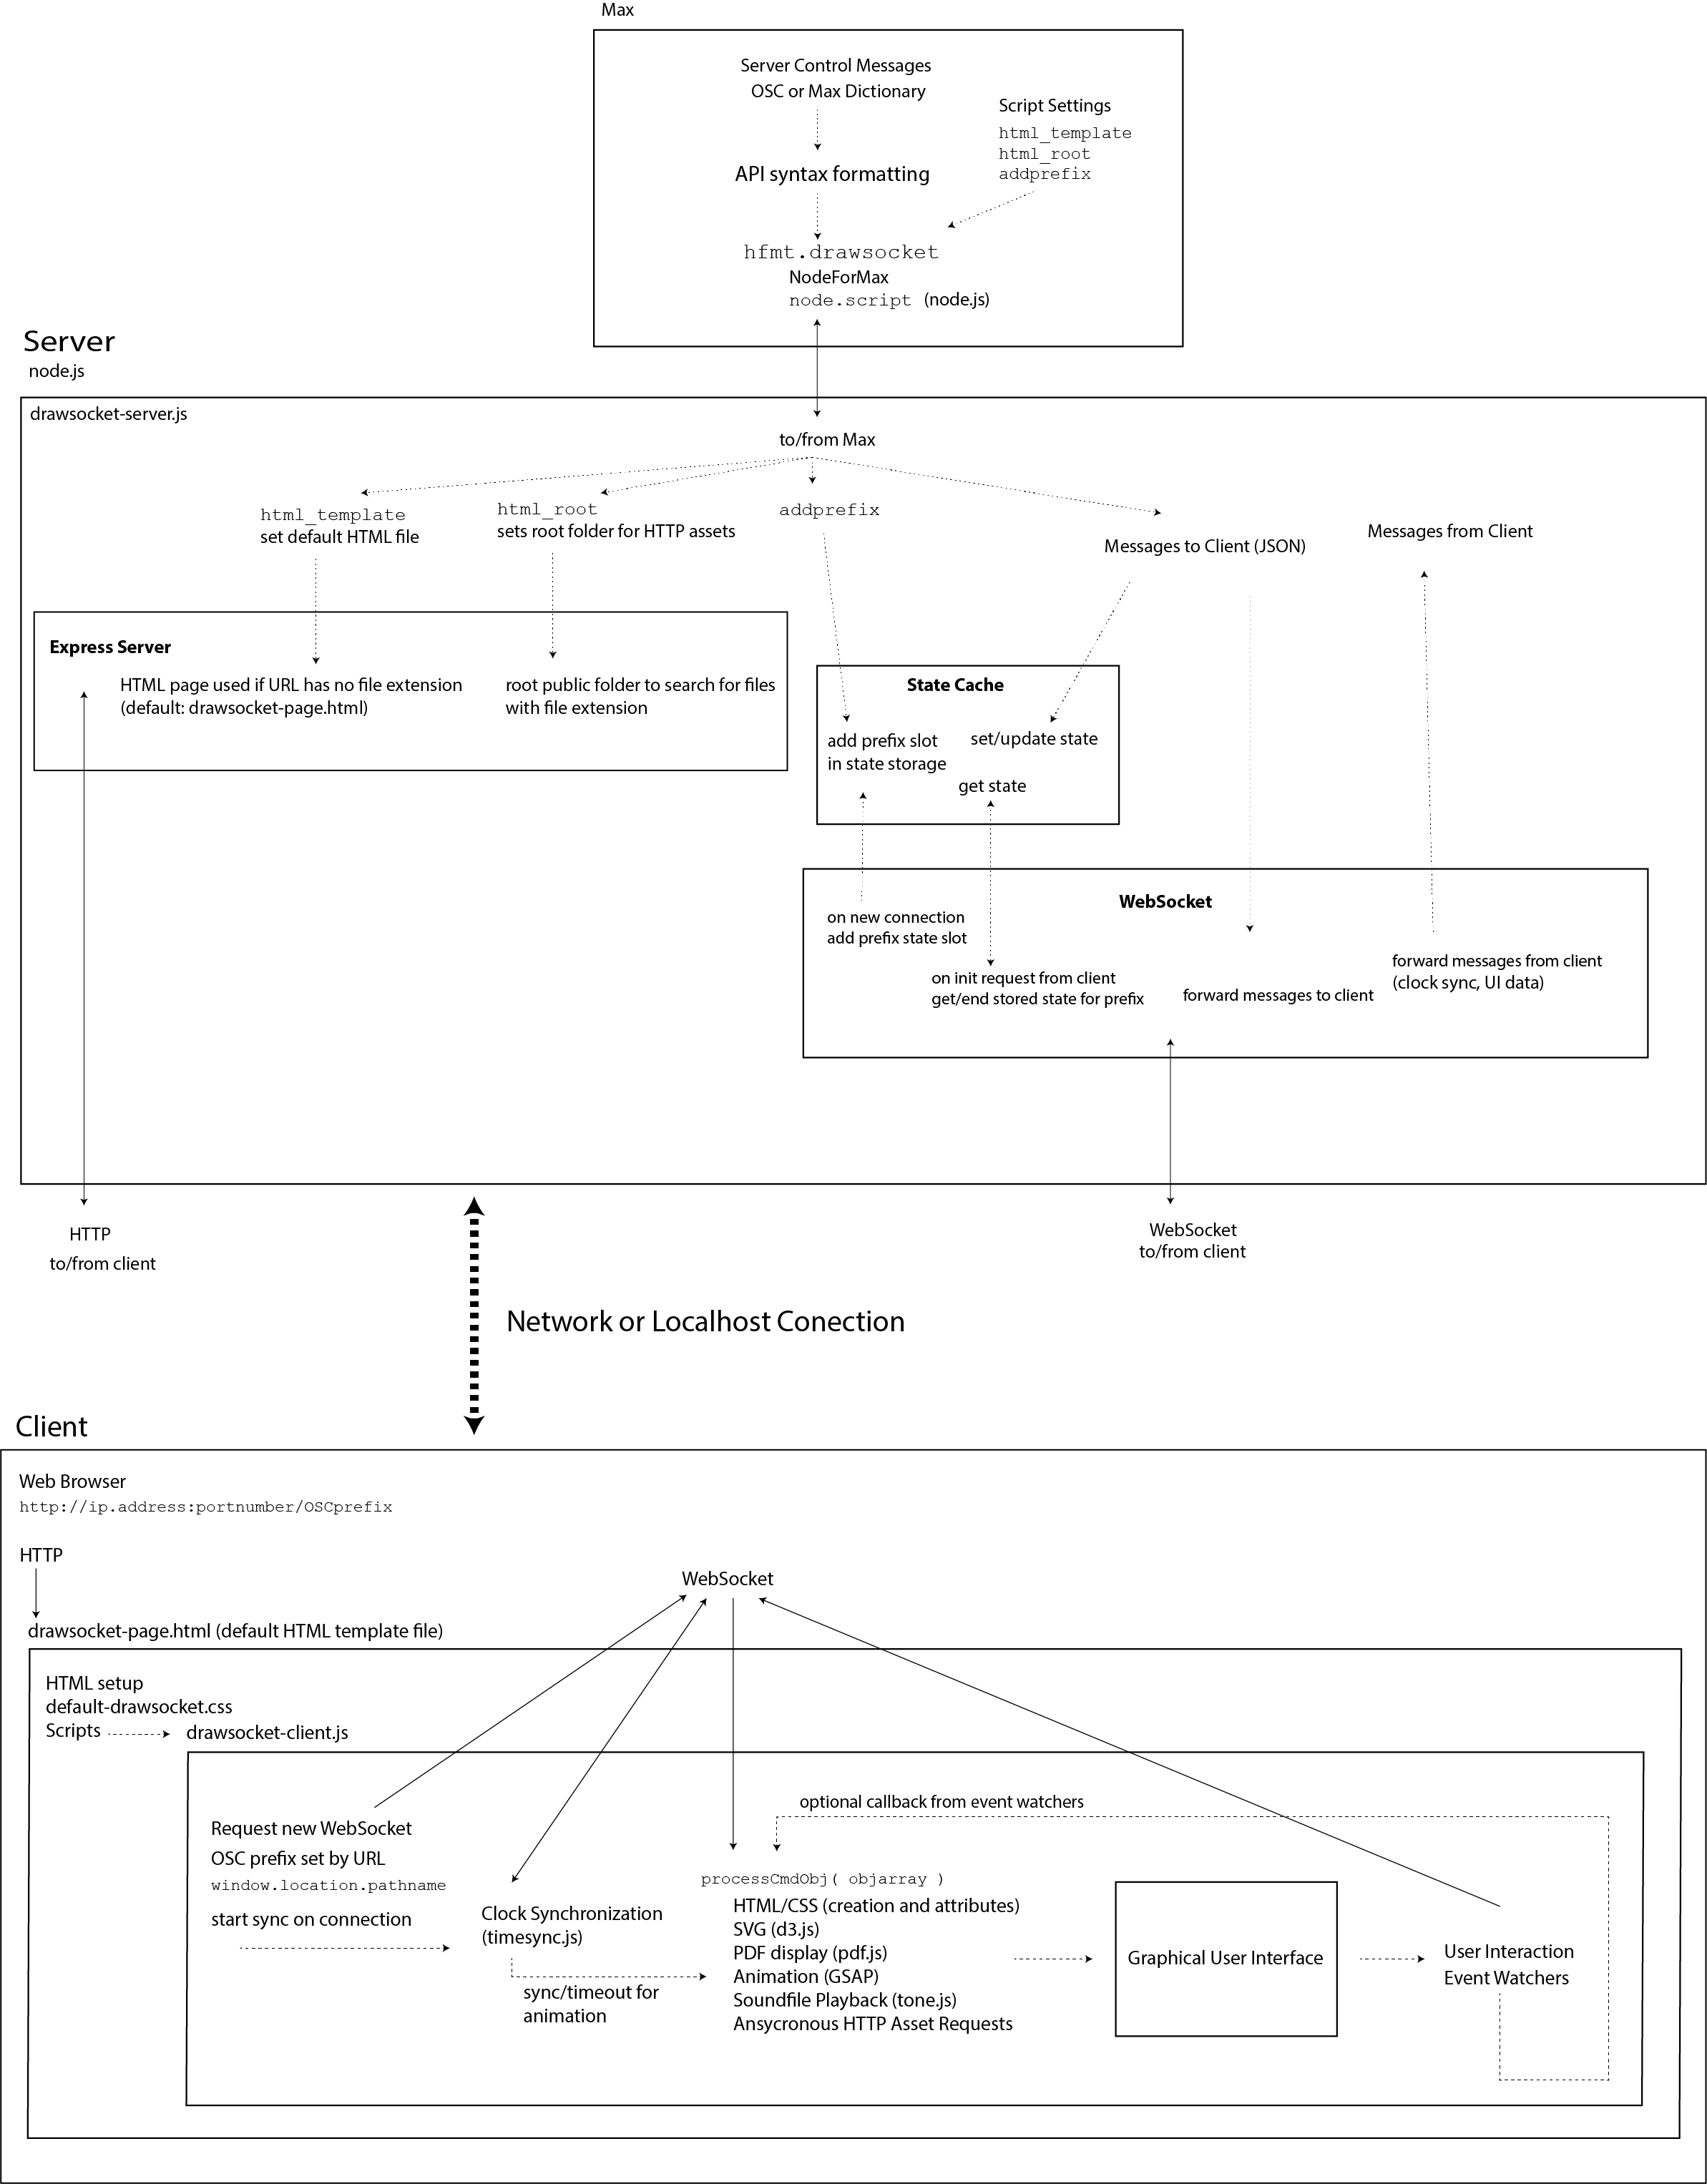
\includegraphics[width=\textwidth]{drawsocket-system.png}
\caption{\drawsocket Server/Client Architecture. 
\label{fig:drawsocket-arch}}
\end{figure*}

\subsection{Architecture Overview}
The \drawsocket architecture is structured as a server-client system, using Max\footnote{https://cycling74.com} as the primary controller interface. 
From Max, control messages are sent to specified client browsers via a Node.js\footnote{https://nodejs.org} server, which routes the messages by a given client addresses.
The messages are then parsed and executed in the client-browser, to generate content or perform other actions.

The choice of Node.js for the server backend was particularly helpful due to the Node Package Manager (NPM), which is bundled with Node.js, allowing \drawsocket to leverage the active community of Javascript library development of tools for browser-based display and inter-computer communication \cite{trockman2018adding}. 
Further, NPM provides a practical method for managing libraries dependancies, via the \textit{package.json} system.

In an effort to scale to larger groups of clients running off of the same server, a loosely defined \textit{model-view-controller} \cite{krasner1988description} pattern is used to separate the processes. 
The server is used primarily to relay and cache the drawing commands, while the drawing implementation is offloaded to the client browsers, which with recent developments in mobile computing have become quite efficient~\cite{halpern2016mobile}.
See figure~\ref{fig:drawsocket-arch} for an overview schematic of the system. 

\subsection{Controller}
\noindent
\textbf{Max.}
Currently the primary targeted user server control platform is Max, which provides many algorithmic and interprocess communications tools. 
Since the release of Max 8, Max now includes the Node For Max (N4M)\footnote{https://docs.cycling74.com/nodeformax/api/} framework, which embeds the Node.js server engine within the Max programming environment, accessible through a set of Max objects.

The first versions of the \drawsocket system used an independent Node.js application running from the command prompt and a User Datagram Protocol (UDP)\footnote{https://tools.ietf.org/html/rfc768} socket to send and receive OSC bundles to and from Max, which were then broadcast to subscribed clients.
However, after comparing benchmarks measuring the roundtrip messaging time between Max and node.js, the N4M system was found to be faster, and so we adopted this platform as the primary use case.
However, the \drawsocket system is well compartmentalized, and so could still easily be reconfigured for use with other control applications.

Within Max, the core Node.js server script, \textit{drawsocket-server.js}, is run within Max's \textit{node.script} object. 
For convenience, the node.script object is wrapped in Max abstraction called \textit{hfmt.drawsocket} which aids in managing server asset paths, and handles user interaction messages returning from the client (see section~\ref{sec:setup} for more details).

\medskip
\noindent
\textbf{OSC-JSON representation.}
The \drawsocket data is formatted as a key-value tree, which in Max can be represented as either OSC, or in Max Dictionary format,
both of which can be easily transformed to JavaScript Object Notation (JSON).\footnote{https://www.json.org/} See section~\ref{sec:api} below for an in-depth description of the \drawsocket messaging syntax.

\subsection{Server}
\noindent
\textbf{Node.js.}
The Node.js server consists of four main processes: (1) an Express HTTP server,\footnote{https://expressjs.com/} (2) a WebSocket\footnote{https://www.npmjs.com/package/ws} connection manager, (3) state caching, and (4) handling messages from the client (either forwarding them to the Max host environment or responding back to client,  as in the case of clock synchronization and on-load initialization).

\medskip
\noindent
\textbf{Express.}
The Express JS library is used to create the web server and handle HyperText Transfer Protocol (HTTP)\footnote{https://www.w3.org/Protocols/} requests from client browsers. 
By default, the server responds to all page requests with a default HTML file which contain the basic setup necessary for most uses of the \drawsocket system, with links to dependency JS libraries, fonts, and a default CSS stylesheet.

If a custom HTML page is desired, users can send the \textit{html\_template} message from the Max interface, to set a new default HTML file.

The Express server uses a static public root folder, which exposes a selected folder path that client browsers may load files from. 
To set the root public folder, users can set the \textit{html\_root} folder path as an initialization argument to the \textit{hfmt.drawsocket} abstraction.

User configuration of the system is described further in section~\ref{sec:setup}.

\medskip
\noindent
\textbf{WebSockets.}
WebSockets are used as the primary server-client communication exchange protocol.
The server accepts WebSocket requests from client browsers, and subscribes clients to receive messages addressed to their browser's URL (Uniform Resource Locator).

Control messages composed in Max as an OSC bundle or Max Dictionary are received in JSON format by the server, and routed to the clients identified by their corresponding URL web-address.\footnote{https://www.w3.org/Addressing/URL/url-spec.txt}

\medskip
\noindent
\textbf{URL state caching.}
Upon receiving control messages addressed to a new URL, the server first forwards the messages via WebSocket to the specified URL address, and then sends a copy of the message to the sate cache system.

On connection to a new WebSocket, the client requests the current state of its URL from the server cache.
This provides a mechanism for preloading a set of drawing commands to a given URL, so that when a user first loads the page, or hits refresh, the current drawing state of the page will be loaded.

\medskip
\noindent
\textbf{Client return messages.}
WebSocket connection is bidirectional, and is used to handle messages from the client: responding to clock synchronization requests, client requests for initialization, and forwarding user interaction information to Max.

\medskip
\noindent
\textbf{Connection Port.} 
On startup, the server provides it's IP address and connection port to the Max environment.
Clients may connect remotely via network IP address, or if on the same computer, use the localhost identifier, followed by the port number (currently 3002 by default), separated by a colon (e.g. \textit{http://localhost:3002}).
 
 \subsection{Client}  
Running inside a web browser, the client-side component of the \drawsocket system handles the drawing and sound generating commands, clock synchronization, and user interface event watchers.

\medskip
\noindent
\textbf{Web browser.}  
Currently the system targets Safari and Chrome.
At the current time of writing, Firefox SVG 2 feature support is behind the above two.
Other browsers will most likely work, but are not currently being tested. 

\medskip
\noindent
\textbf{Layout.}
The central browser display layout consists of one HTML \textless div\textgreater\ node, which contains an \textless svg\textgreater\ element, and an SVG \textless g\textgreater\ group node. 

\begin{lstlisting}[
  mathescape,
  columns=fullflexible,
  basicstyle=\oscfontsize\fontfamily{lmvtt}\selectfont ]
 <div id=``main-div''>
    <svg>
         <defs id=``defs''></defs>
         <g id=``main-svg''></g>
    </svg>
 </div>
\end{lstlisting}

The default formatting for the basic page elements is setup in the \textit{drawsocket-defaults.css}.
When users add SVG elements, they are added to the ``main-svg'' group.
Users may also create new SVG groups and add elements to these new groups, to control stacking order, described below in more detail.

\medskip
\noindent
\textbf{Libraries.}
\drawsocket currently makes use of the following client-side Javascript libraries, all available from NPM:

{D3.js},\footnote{https://d3js.org/} a library for SVG information visualization.\footnote{We are now mainly using d3.js for DOM node creation and manipulation. So, eventually it is likely that we will remove the d3.js dependency to streamline the codebase. However for the time being d3's utility functions are convenient for rapid development, and appear to be performant enough.}

{PDF.js},\footnote{https://mozilla.github.io/pdf.js/} a PDF viewer library developed by Mozilla, providing support for PDF file reading, viewing and page turning.

{Tone.js},\footnote{https://tonejs.github.io} a web-audio library by Yotam Mann. Currently, \drawsocket uses Tone.js to provide basic soundfile playback functionality, this may be expanded in the future.

{Timesync.js},\footnote{https://www.npmjs.com/package/timesync} a clock synchronization library, used in \drawsocket to synchronize animations, and provide a mechanism for timed commands.

 {TweenMax} and {TimelineMax}, from the GreenSock Animation Platform (GSAP),\footnote{https://greensock.com/gsap} a high-performance system for JS and CSS animation.
%
%\begin{figure*}[]
%\centering
%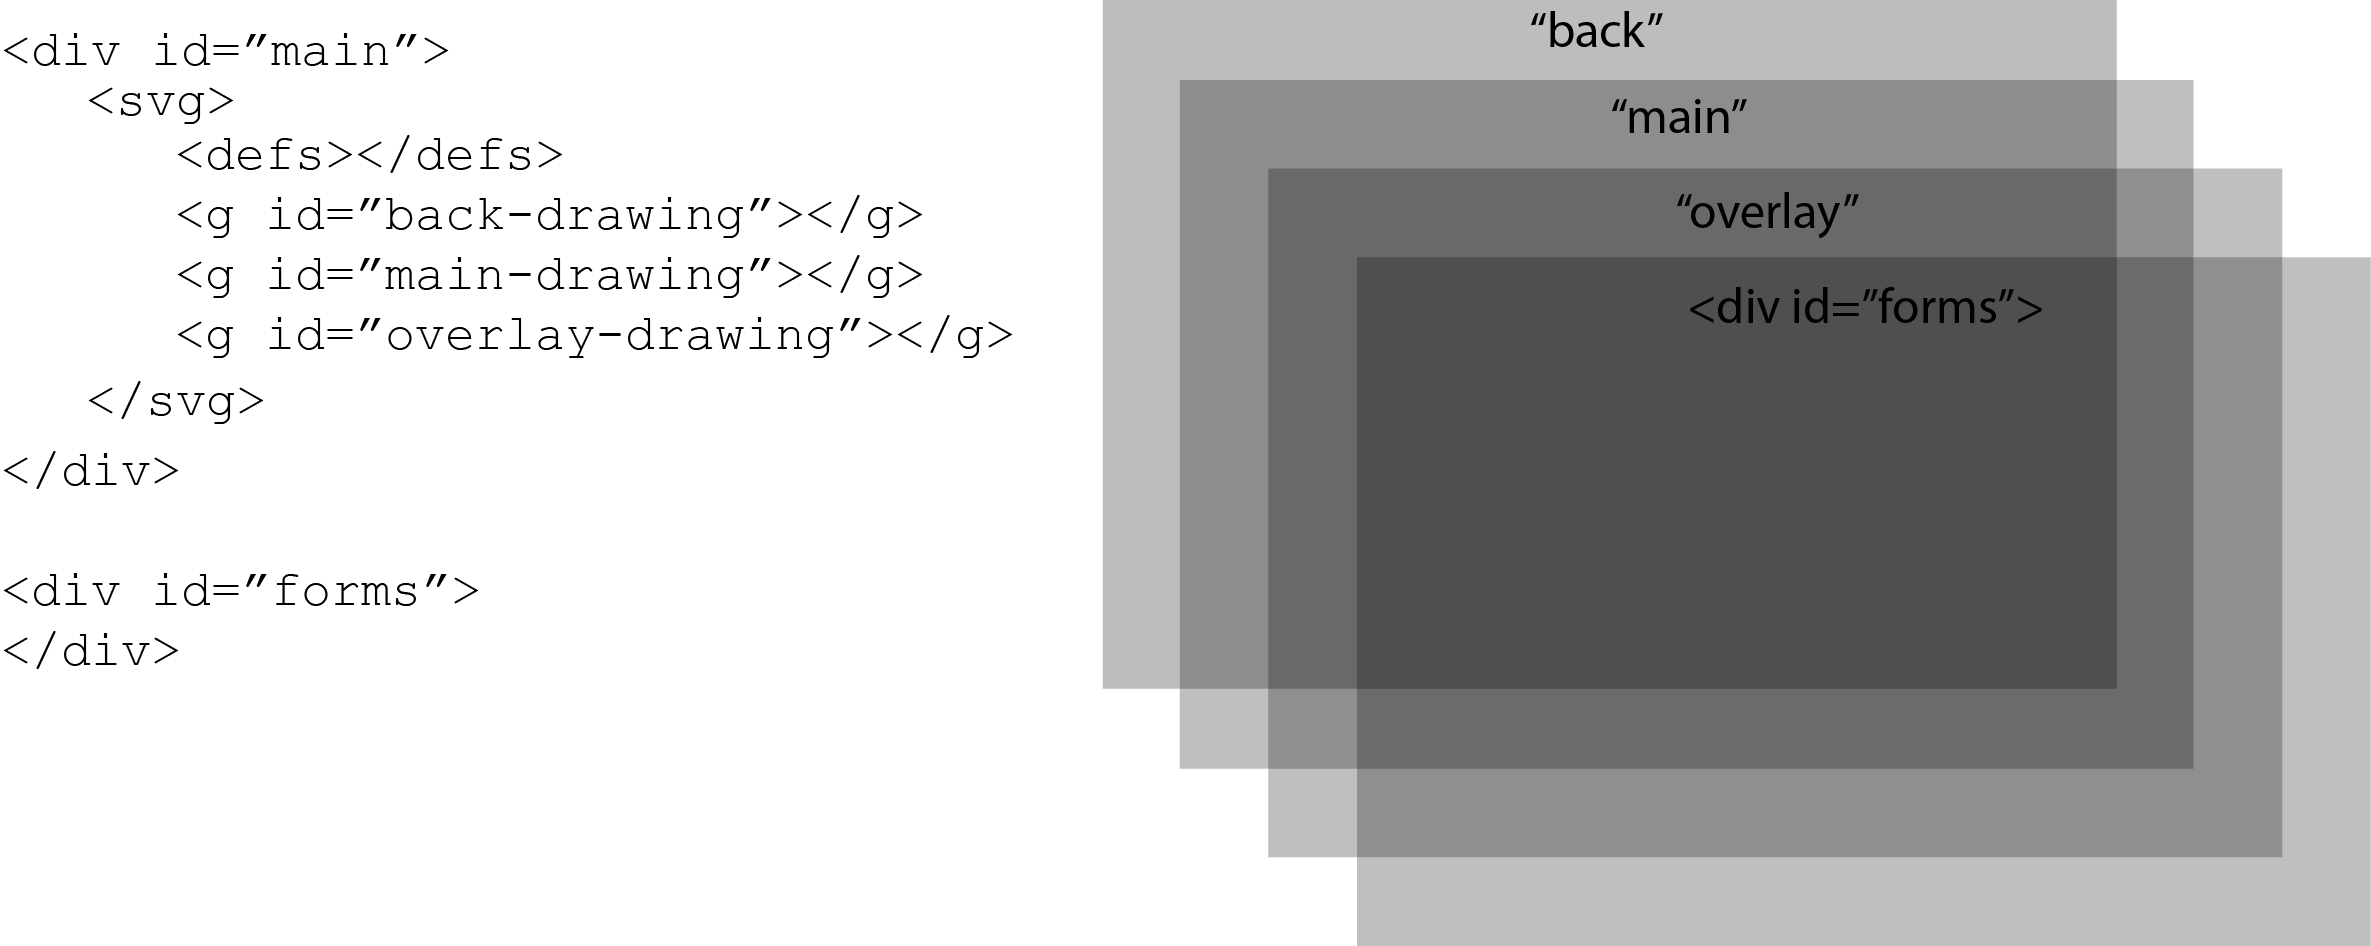
\includegraphics[width=0.75\textwidth]{display-layers.png}
%\caption{\drawsocket display layers. 
%\label{fig:drawsocket-layers}}
%\end{figure*}
%

\medskip
\noindent
\textbf{Client-side Script.} 
The client-side script running in the browser is called \textit{drawsocket-client.js}, which handles the command processing logic of the system and its execution in the browser.

On load, the script first requests a new WebSocket connection to the server using the browser's URL address, sent to the server via the the WebSocket URL identifier (e.g. \textit{ws://localhost:3002/violin}). On successful WebSocket connection, the script begins the clock synchronization process which runs in the background on the client system, requesting new clock readings from the server at regular intervals\footnote{Currently, the script is configured to check every 5 seconds, but this may change depending on performance on a larger scale system}. Once the initial clock synchronization is completed, the script sends a state initialization request to the server, to which the server responds with a sequence of commands corresponding to the current state of the given client OSC address.

The central command processing is performed in the function \textit{drawsocket}, which parses an array of time-tagged command objects, and executes the corresponding graphic and sound manipulations in the browser. The \textit{drawsocket} function expects one or more objects with a \textit{key}, \textit{val}, and \textit{timetag} key-value pairs:

\begin{lstlisting}[
  mathescape,
  columns=fullflexible,
  basicstyle=\oscfontsize\fontfamily{lmvtt}\selectfont ]
  {
      timetag: current time (supplied by server),
      key: command string
      val: command arguments
  }
\end{lstlisting}
\noindent
Generally, these objects are formatted in the Node.js server from the API command messages received via Max, however they may also be created by user scripts called from event watchers.

%%%%%%%% User Setup
\section{Drawsocket User Setup}\label{sec:setup}
The interface for \drawsocket is designed for use in Max, and is distributed as a Max Package, currently hosted on GitHub at the following url:

\textit{https://github.com/HfMT-ZM4/drawsocket}

To install, users download the repository and place it in Max's Packages folder. Once installed, users can instantiate the \drawsocket system by creating a hfmt.drawsocket object in a Max patch.

The dependency NPM libraries are not distributed with the package, so on first loading hfmt.drawsocket, you need to send the object the \textit{``script npm install''} message, which asks NPM to download all of the dependencies listed in the node project's \textit{packages.json} file.\footnote{The node project is located in the package's /code/node folder, and includes all scripts, and configuration files.}

\medskip
\noindent
\textbf{Setting the public folder.}  As mentioned above, by default the \drawsocket server responds to HTTP URL page requests with a default HTML page. 
Custom HTML pages, and/or other types of assets can also be served to the client from a static root public folder. 

The public root folder is a method commonly used to control client access to server folders, and can be set in Max by supplying the relative path to the user's Max patch\footnote{Note that the Max patch must be saved to disk before it will have a valid folder path.} as an argument to the hfmt.drawsocket object.
This system allows users to organize their project in a mobile way, easily moved or installed on a new system.

Within the hfmt.drawsocket abstraction there is a helper script called \textit{startscript.js} which retrieves the user patcher's folder path, and passes the path information as an argument to the node.script object on startup.\footnote{Note that this requires the user patcher to be saved to disk first, so that it has a valid folder location.}
By default the folder containing the user's patch is used as the root public folder, however, users may wish to choose a different folder. 
For example, by setting the path ``public\_html'', \drawsocket will expect a folder called ``public\_html'' to be located in the same folder as the Max patch running the hfmt.drawsocket abstraction, and if found will use this folder as the public root folder.

In larger projects it is often convenient to sort assets into separate folders for images, sound files, etc. For example if the user wishes to load an image file called ``foo.jpg'' located in a \textit{/public\_html/images} subfolder, they would refer to their file at the address \textit{/images/foo.jpg}.

%%%%%%%% API
\section{Drawsocket API}\label{sec:api}
The \drawsocket API has developed organically as features are gradually added to the system, and has been rewritten several times as new use contexts have arisen.

The API was initially designed in keeping with the conventional ``message'' format used in the Max environment, so that drawing commands could be easily adapted from commands used for other Max drawing objects such as LCD, or jit.gl.sketch.

A Max message is structured as an array, beginning with a selector string, followed by a list of values, which is interpreted by the receiver based on a preexisting schema.
However, as more features were added, some complications arose in regard to the sequence ordering, and as a result an alternative object-oriented API was developed, which makes use of a key-value approach that has proven more extendable for the \drawsocket system (discussed below in section~\ref{sec:objstyle}).

Note that in the discussion below, we use the term \textit{message} as a general purpose term for communication via message events, which could be in different formats (OSC messages, Max messages, JSON objects sent as messages, etc.).


\medskip
\noindent
\textbf{URL address routing.}  
All messages sent to the server are addressed to a URL, which is used by the server to route messages to the appropriate clients. 
Multiple clients may be logged into the same URL, in which case they would all receive the same drawing commands. 
For example if you had a group of violins all playing the same part you could have them log into the URL:

\textit{http://server.ip.address:port/violin1}

Then to send messages to the violin 1 section, you would use the URL address \textit{/violin1}, in the same way you wold use an OSC address.

To send to all clients, regardless of URL address, \drawsocket provides usage of the OSC \textit{/*} wildcard address.

Note that in OSC, \textit{/*} matches one single address level, whereas the \drawsocket server uses the wildcard address to match any \textit{URL}, which may include multiple slashes.
To avoid confusion with OSC convention, it is strongly recommended to use single level addresses (i.e. use \textit{/violin1}, not \textit{/violin\textbf{/}1} in cases of indexed sub-groupings).

\medskip
\noindent
\textbf{Object references.} 
\drawsocket uses the Document Object Model (DOM)\cite{Champion:04:DOM} \textit{id} attribute as the primary mechanism for referencing individual client objects from the server.
On creation, the client-side script logs a reference to new objects with their unique ID, in a set of associative arrays which can be used for fast object lookup by name. 
Through this method, objects may be referred to by ID, modified, styled, transformed, or removed.

SVG and HTML nodes use the provided unique identifier as the node's \textit{id} attribute, as per the DOM standard, while other objects such as GSAP animation or Tone.js sound objects are not in the DOM, but logged in the \drawsocket's internal object model.

\subsection{List-oriented API}\label{sec:maxstyle}
The original ``Max style'' list-oriented  \drawsocket API design used a bundle of individual OSC messages, each of which performed an action on the client system. 
The list-oriented API has now been replaced, however a discussion of this approach is valuable, since it illustrates a structural limitation that we encountered with this syntax approach.

In the list-oriented API, the OSC message address was used as a way to specify several functional layers at once, through concatenating together multiple values separated by slashes. The general address syntax was made of three main levels: (1) the client URL address, (2) a unique object ID, followed by (3) a command string specifying the process to execute on the client system.

The commands provided a streamlined way to create and modify elements on the client browser, using a curated set of parameters. 

For example the following OSC bundle:

\begin{lstlisting}[ mathescape,columns=fullflexible,basicstyle=\oscfontsize\fontfamily{lmvtt}\selectfont ]
    {
         /violin/foo/draw/rect : [100, 100, 25, 25],
         /violin/foo/style/stroke-width : 1
    }
\end{lstlisting}

\noindent
contains two messages prefixed by \textit{/violin} which indicates that the server should send these commands to all clients logged into the \textit{/violin} URL.

Once received on the client system, the script would parse the OSC address, separating the ID from the command string. 
Here, the ID is ``foo'' and the command string is ``draw/rect''.

For each OSC message, the value attached to address was parsed by the client script based on schema defined in the documentation.
In the case of ``draw/rect'', the message's value would be interpreted as defining an SVG rectangle's \textit{x},  \textit{y},  \textit{width}, and \textit{height} values.
The second message works in a similar way, except that rather than creating a new object, it adds an inline SVG/CSS \textit{style} attribute to the object node, setting the \textit{stroke-width} parameter to a value of 1.

\medskip
\noindent
\textbf{Grouping.} 
Things start to get a little more complex with the list-oriented approach when attempting to define SVG group objects and object definitions. 
In these cases child objects can be grouped together and manipulated as a single graphic object, while not requiring each child object to have a unique ID.

The first problem we encountered was when trying to include two objects of the same type within the object. 
In the first implementation, a sub-bundle of OSC messages was used to group elements together, however since no IDs were required, the following example fails:

\begin{lstlisting}[ mathescape,columns=fullflexible,basicstyle=\oscfontsize\fontfamily{lmvtt}\selectfont ]
    /*/groupex/draw/group : {
	/text : [210, 210, ``hi''],
	/text : [310, 210, ``bye'']
    }
\end{lstlisting}

\noindent
It fails because in OSC you are allowed to have multiple messages with the same address, however in Max the OSC messages need to be first converted to Max Dictionary format to be passed to the node.script object, and Max Dictionaries do not allow duplicate addresses.

Another complication arose when trying to style individual objects within a group, since there is no unique identifier to reference for adding inline style tags, and this is not accessible from the list-oriented API syntax. 
To address these two issues, the list-oriented grouping syntax was adapted to use an array of objects (aka sub-bundles in OSC). For example:
 
\begin{lstlisting}[ mathescape,columns=fullflexible,basicstyle=\oscfontsize\fontfamily{lmvtt}\selectfont ]
    /*/groupex/draw/group : [{
	/path : ``M200,200a30,90,0,0,0,0-60a30,30,0,0,0,0,60'',
	/style : ``fill: black''
    }, {
	/text : [210, 210, ``hi''],
	/style : ``fill: red''
    }]
\end{lstlisting}

\noindent
In this case, the \textit{style} message is bound to the \textit{path} message by wrapping them together in an object. 
This solution led to a reevaluation of the \drawsocket API syntax, and resulted in the development of the object-oriented based API.

\subsection{Object-oriented API}\label{sec:objstyle}
While the list-oriented approach provides a compact, one-line syntax, the list format is also limited, in that the list requires a predefined schema for how the list can be interpreted, and which types of operations the list values may address. 
The list-based approach is thus less easily extendable, since adding a new value to the list requires adding a new step in the interpreting script.
The main benefit of the list syntax is that its compactness makes it sometimes faster for rapid prototyping, however the object-oriented approach can be more easily expanded as we will show below, and additionally, the object-oriented approach is helpful since it is self-describing, emphasizing legibility by associating a parameter name with each value.

%The ``object-array'' API uses an array of objects which are processed in a similar way to the ``list-oriented'' API, except that rather than concatenating the sequence of \textit{id}, \textit{command}, and associated generic list of values that need to fit a certain order to be interpreted correctly by the client-side script, the object-oriented approach groups all parameters together in an object and provides separate identifiers for each element. 

For example, whereas above we drew a rectangle with a list, such as:
\begin{lstlisting}[ mathescape,columns=fullflexible,basicstyle=\oscfontsize\fontfamily{lmvtt}\selectfont ]
  /violin/foo/draw/rect : [100, 100, 25, 25]
\end{lstlisting}

\noindent
The same rectangle could be drawn with the object-based API using the ``svg'' \textit{key}, and an \textit{val} containing one or more objects to process. The \textit{``new''} keyword notifies the client that it should create a new SVG element:

\begin{minipage}{\linewidth}
\begin{lstlisting}[ mathescape,columns=fullflexible,basicstyle=\oscfontsize\fontfamily{lmvtt}\selectfont ]
  /violin : {
    /key : "svg",
    /val : {
        /new : ``rect'',
        /id : ``foo'',
        /x : 100,
        /y : 100,
        /width : 25,
        /height: 25
      }
  }
\end{lstlisting}
\end{minipage}

\noindent
In the object-based approach each variable now has a name associated with its value, telling us what the variable represents.
The list-approach is a more concise, requiring less typing, however, when we consider further what the messages are representing in the context of the \drawsocket system, the benefit of the object approach becomes clearer.

SVG is based on the Extensible Markup Language (XML)\footnote{https://www.w3.org/TR/xml/} format, and is designed as tree of \textit{nodes}, each with a set of \textit{attributes} which are defined as key-value pairs.
By using the same attribute names within the \drawsocket object API, the client script can then simply insert as few or many of the attributes as it receives, rather than needing a specific set of attributes, as with the list-based approach.
Also, by staying close to the original SVG API, the user can refer to the SVG specification directly to figure out which attributes they can use, rather than needing to limit their control parameters to those setup in the list parsing schema.\footnote{That said, we have not yet fully tested the entire SVG specification. We believe the object API provides access to everything, but there maybe some unaddressed aspects.} 


For example, extending the above example, here we create two new objects, a rectangle and a circle, by defining them in an array, and additionally assign a CSS \textit{class} reference for each:

\begin{minipage}{\linewidth}
\begin{lstlisting}[ mathescape,columns=fullflexible,basicstyle=\oscfontsize\fontfamily{lmvtt}\selectfont ]
  /violin : {
    /key : "svg",
    /val : [{
      /new : ``rect'',
      /id : ``foo'',
      /x : 100,
      /y : 100,
      /width : 25,
      /height: 25,
      /class : ``room''
    }, {
      /new : ``circle'',
      /id : ``bar'',
      /cx : 112,
      /cy : 112,
      /r : 5,
      /class : ``source'
    }]
  }
\end{lstlisting}
\end{minipage}

%The \drawsocket object API uses the native SVG attributes by name as per the SVG specification, with the addition of the \textit{new} keyword.

\medskip
\noindent
\textbf{Keywords.} 
There are currently four reserved keywords used with \textit{svg} objects: \textit{new}, \textit{style}, \textit{parent}, and \textit{child}.

On receiving an \textit{svg} object (or array of objects), the client-side script iterates each element of the array, and checks if there is an already existing object with that \textit{id} tag; if so, it selects that element from the DOM lookup table.
Next, the script checks if there is a \textit{new} message in the object; if so, it creates a new node, either replacing the element at the existing \textit{id}, or creating a new node if not already existing, and then processes the rest of the object messages.

If the object already exists, and no \textit{new} is found, \drawsocket will use the values in the object to update the object attributes. For example:

\begin{minipage}{\linewidth}
\begin{lstlisting}[ mathescape,columns=fullflexible,basicstyle=\oscfontsize\fontfamily{lmvtt}\selectfont ]
/violin : {
    /key : "svg",
    /val : {
      /id : ``foo'',
      /width : 100
    }
}
\end{lstlisting}
\end{minipage}

\noindent
will change the \textit{width} attribute of the node ``foo'' without modifying any other attributes that may have already been set.

\subsection{Parent and child elements}\label{sec:parent}
Appending child nodes to parent SVG element can be accomplished via the \textit{parent} and \textit{child} keywords.

The \textit{child} keyword, is a high-level API helper function that assists the user in specifying one or more child nodes in a tree syntax.
The value attached to this address will be inserted as a child of the parent node, for example the inner text of a \textless text\textgreater element, or a new node within a \textless g\textgreater the SVG grouping element tag.

Here is an example of a circle and line contained in new SVG group, called ``noteline'':

% osc data formating
\begin{lstlisting}[ mathescape,columns=fullflexible,basicstyle=\oscfontsize\fontfamily{lmvtt}\selectfont ]
/violin : {
    /key : "svg",
    /val : {
        /new : ``g'',
        /id : ``noteline'',
        /x : 100,
        /y : 100,
        /child : [{
      	    /new : ``line'',
            /id : ``liney'',
      	    /x1 : 10,
      	    /y1 : 5,
      	    /x2 : 100,
      	    /y2 : 5,
      	    /style : {
      	        /stroke-width : 1
      	    }
      	}, {
      	    /new : ``circle'',
            /id : ``circley'',
      	    /cx : 5,
      	    /cy : 5,
      	    /r : 5,
      	    /style : {
      	        /stroke-width : 2,
      		/fill : ``none'',
      		/stroke : ``black''
      	    }
        }]
     }
  }
\end{lstlisting}

Nodes with a \textit{parent} attribute are inserted as children of the node with the \textit{id} specified by the \textit{parent}, as long as the parent element is already existing in the DOM.
If no \textit{parent} element is specified, the node is inserted into the default SVG group ``main-svg''.

\begin{minipage}{\linewidth}
For example, the above tree syntax could also be written this way:

\begin{lstlisting}[ mathescape,columns=fullflexible,basicstyle=\oscfontsize\fontfamily{lmvtt}\selectfont ]
 /violin : {
    /key : "svg",
    /val : [{
        /new : ``g'',
        /id : ``noteline'',
        /x : 100,
        /y : 100
   }, {
        /new : ``line'',
        /id : ``liney'',
        /parent : ``noteline'',
        /x1 : 10,
        /y1 : 5,
        /x2 : 100,
        /y2 : 5,
        /style : {
            /stroke-width : 1
      	}
   }, {
        /new : ``circle'',
        /id : ``circley'',
        /parent : ``noteline'',
        /cx : 5,
        /cy : 5,
        /r : 5,
        /style : {
            /stroke-width : 2,
            /fill : ``none'',
            /stroke : ``black''
        }
    }]
 }
\end{lstlisting}
\end{minipage}


\subsection{SVG layer drawing contexts}\label{sec:contexts}
In an SVG file, each object element is drawn in the same order as they are written in the file, from top to bottom, with the last element being drawn last, ``on top'' of any objects that may have been drawn in the same location.
In the \drawsocket system, the drawing sequence is set through the order of the object creation (using the \textit{new} keyword).

Using the \textit{parent} and \textit{child} keywords, new nodes can be created and inserted as children of existing nodes.
The order in which the child nodes are created, sets the drawing order of the nodes.
Importantly, \textit{editing} nodes (i.e. setting values without the use of the \textit{new} keyword), does \textit{not} change the drawing order.
Similarly, inserting nodes does not change the drawing order of the parent nodes.
This rule makes it possible to use SVG groups as drawing layer contexts, which maintain stacking order relative to each other.

As an illustration, let's say you would like to have three layers, a background, middle and overlay. 
You could create three new groups within the main SVG node, called ``back'', ``main'', and ``overlay'', in a specific drawing order, like this:

\begin{lstlisting}[ mathescape,columns=fullflexible,basicstyle=\oscfontsize\fontfamily{lmvtt}\selectfont ]
 /violin : {
    /key : ``svg'',
    /val : [{
       /new : ``g'',
       /id : ``back''
     }, {
       /new : ``g'',
       /id : ``main''
    } , {
       /new : ``g'',
       /id : ``overlay''
   }]
 }
\end{lstlisting}

You could then use the \textit{parent} keyword to append nodes to the newly created groups. New nodes are draw above older nodes, but since the groups maintain their drawing order, you can use them as layers. In this example, the ``overlay'' layer, will always be drawn after the ``back'' and ``main'' layer-groups.

\begin{minipage}{\linewidth}
\begin{lstlisting}[ mathescape,columns=fullflexible,basicstyle=\oscfontsize\fontfamily{lmvtt}\selectfont ]
  /* : {
        /key : ``svg'',
        /val : [{
            /parent : ``main'',
            /id : "clef",
            /new : "text",
            /child : "&#xE050",
            /class : "bravura_text",
            /x : 40,
            /y : 50
        }, {
            /parent : ``back'',
            /new : "rect",
            /id : "rect",
            /x : 5,
            /y : 5,
            /width : 100,
            /height : 100,
            /fill : "red"
        }, {
            /parent : ``overlay'',
            /new : "circle",
            /id : "circle",
            /cx : 50,
            /cy : 50,
            /r : 10,
            /fill : "blue"
        }]
  } 
\end{lstlisting}
\end{minipage}

Using this approach, multiple layers of SVG elements can be grouped together and manipulated (with some limitations as described in the SVG specification).

\subsection{SVG CSS Styling.} 
The ability to dynamically apply CSS styling operations on SVG elements provides the user with an extremely flexible mechanism for composing, and manipulating the graphic layout.
For most common \drawsocket usages, a set of default layout properties are defined in the file \textit{drawsocket-default.css}, which is loaded with the default HTML file (\textit{drawsocket-page.html}).
The linked stylesheet sets some defaults for SVG element types, for example \textit{lines} have a default stroke width value so that they are visible by default.\footnote{Note that this is not always desirable, for example when importing SVG files exported by a program like Adobe Illustrator, which assumes that there are no pre-exiting CSS rules in place. For these cases, \drawsocket users can either override the defaults via a new CSS definition, or change the .css file by hand.}

\drawsocket also provides dynamic access to CSS rules, for which it is useful to understand the hierarchy of SVG style properties. 

There are three levels of inheritance with SVG CSS styling: 

(1) \textit{presentation attributes}, set within the element, e.g.:

\textit{\textless rect~fill=``red''~\textgreater}; 

(2) \textit{stylesheet} definitions, loaded via an attached CSS stylesheet document, or within an \textless style\textgreater element within the HTML document;
and

(3) \textit{inline styling}, a snippet of CSS wrapped in a string and set in an elements's \textit{style} attribute, e.g.:

\textit{\textless rect~style=``fill:~red;~stroke:~2''~\textgreater}.

Each is overridden by the next: stylesheets override presentation attributes, and inline styles override all the others.\footnote{With one exception, stylesheet definitions with the \textit{!important} tag will override inline styles.} 

Using CSS \textit{class} selector syntax opens up many possibilities.
For example, here is an example using the object-array syntax to set create two CSS classes: (1) ``.notehead'' which sets defaults for fill and stroke properties, as well as the radius value, \textit{r} ; and (2) ``.notehead.open'', a sub-class of ``.notehead'' which overrides the fill property. 

Following the \textit{css} definitions, a new SVG circle object is created and configured with the ``notehead open'' class.

\begin{lstlisting}[ mathescape,columns=fullflexible,basicstyle=\oscfontsize\fontfamily{lmvtt}\selectfont ]
 /violin : [{
    /key : ``css'',
    /val : [{
      /selector : ".notehead",
      /props : {
          /stroke : "black",
	  /stroke-width : 2,
	  /fill : "black",
          /r : 5
      }
    }, {
      /selector : ".notehead.open",
      /props : {
          /fill : "none"
      }
    }],
  }, {
    /key : ``svg'',
    /val : {
       /new : ``circle'',
      /id : ``foo'',
      /class : ``notehead open'',
      /cx : 20,
      /cy : 20
    }
  }]

 \end{lstlisting}


\subsection{SVG import and library definitions}\label{sec:defs}
\drawsocket provides access to several methods for importing and reusing fragments of SVG.
This is a useful approach for reducing the amount of data that needs to be sent over the network, and can greatly simplify the construction of more complex notation situations.

\medskip
\noindent
\textbf{Referencing SVG definitions.} 
There are two node types in the SVG specification which allow the user to create prototypes of graphic elements, \textit{defs} and \textit{symbol}, which can be applied like a stamp via the \textit{use} tag. 

Within the \drawsocket main SVG element there is element group called \textit{defs} which is not directly drawn to the screen, but is visible by using the browser's HTML element viewer tool.
\drawsocket uses the same drawing context syntax for the \textit{defs} node, as it does for the other drawing layers.

For example, the following snippet makes a new SVG group object in the \textit{defs}, called ``noteline'', which contains a line and a circle:

\begin{minipage}{\linewidth}
\begin{lstlisting}[ mathescape,columns=fullflexible,basicstyle=\oscfontsize\fontfamily{lmvtt}\selectfont ]
 /violin : {
    /key : ``svg'',
    /val : {
      /parent : "defs",
      /new : ``g'',
      /id : ``noteline'',
      /child : [{
          /new : ``line'',
          /x1 : 10,
          /y1 : 10,
          /x2 : 100,
          /y2 : 10
       }, {
        /new : ``circle',
        /cx : 5,
        /cy : 5,
        /r : 5
      }]
    } 
  }
 \end{lstlisting}
 \end{minipage}

Typically the user would send a library of definitions at the beginning of the piece, and then refer to the set of definitions as needed via the \textit{use} SVG element and its \textit{href} attribute, creating an internal reference to a given definition selected through its \textit{id} attribute.\footnote{Note that for all selections we are using the HTML/CSS \textit{\#} sign to specify that the following string is an \textit{id}.}

For example, the following new SVG object ``foo'', references the ``noteline'' definition above, offset to ${x,y}$ position $\{100,100\}$:

\begin{minipage}{\linewidth}
\begin{lstlisting}[ mathescape,columns=fullflexible,basicstyle=\oscfontsize\fontfamily{lmvtt}\selectfont ]
 /violin : {
    /key : ``svg'',
    /val : {
      /new : ``use'',
      /id : ``foo'',
      /href : ``#noteline'',
      /x : 100,
      /y : 100
   }
 }
 \end{lstlisting}
\end{minipage}

\medskip
\noindent
\textbf{Importing fragments.} 
The \textit{use}-\textit{href} syntax approach can also be used to import elements from external SVG files stored in the public HTML folder, by adding the target object's \textit{id} to the external file path.
For example, to reference an object with the ID ``boo'' in an external file called ``other.svg'' that is located in the public subfolder called ``media'' you could use the following snippet:

\begin{lstlisting}[ mathescape,columns=fullflexible,basicstyle=\oscfontsize\fontfamily{lmvtt}\selectfont ]
 /violin : {
    /key : ``svg'',
    /val : {
      /new : ``use'',
      /id : ``foo'',
      /href : ``/media/other.svg#boo''
   }
 }
 \end{lstlisting}

If \textit{x} or \textit{y} attributes are set in the \textit{use} node, the referenced object will be offset by the amount specified by the  \textit{use} attributes.

\drawsocket also provides an additional option with the \textit{href} attribute. If the \textit{href} value is a list, the second value is non-zero, the script will find the original object's bounding box and offset so that it lies at the origin $\{0,0\}$, and then applies the ${x,y}$ values as a second operation. The benefit of this feature is that it allows you to coordinate positions of objects without needing to know their original position in the reference file.

\subsection{PDF import}\label{sec:pdf}
PDF files may be imported into \drawsocket.
For example, to load a PDF, storing it at the \drawsocket ID ``foo'', setting its \textit{x} position, \textit{width} and setting it to display page 2:

\begin{lstlisting}[ mathescape,columns=fullflexible,basicstyle=\oscfontsize\fontfamily{lmvtt}\selectfont ]
  /* : {
     /key : ``pdf'',
     /val : {
      /id : "newpdf",
      /href : "/media/flint_piccolo_excerpt.pdf",
      /width : 600,
      /x : 100,
      /page : 2
    }
  }
 \end{lstlisting}


\subsection{Animation}\label{sec:animation}
While \drawsocket objects may be animated using native CSS transitions and keyframes, the GSAP TweenMax and TimlineMax libraries were introduced to provide a much more convenient and cross-browser supported method.
With the TweenMax library users can create a ``tween'' transition between the object's current position and current CSS property values, to another set of values over a given amount of time, using the TweenMax.to function via the \textit{tween} \drawsocket key. For example:
\begin{lstlisting}[ mathescape,columns=fullflexible,basicstyle=\oscfontsize\fontfamily{lmvtt}\selectfont ]

 /violin : {
    /key : ``tween'',
    /val : {
      /id : ``aaa'',
      /target : ``#note'', 
      /dur : 10,
      /vars : {
        /x : 100,
        /y : 100,
        /opacity : 0
      }
    }
  }
 \end{lstlisting}
\noindent
moves the SVG object ``note'' to the ${x,y}$ positions $\{100,100\}$, and fades the opacity to zero over a course of 10 seconds.
The \textit{tween} is stored as object in the \drawsocket script at the given ID (here ``aaa''), and may be recalled at will (see the online documentation for more details).
The CSS selector \textit{target}, \textit{dur} and \textit{vars} are plugged directly into the argument fields for the TweenMax.to function.\footnote{https://greensock.com/docs/TweenMax/TweenMax()}

More complex animations can be implemented with the TimelineMax function, via the \drawsocket \textit{timeline} command, which is comprised of an array of tweens (which can also have different targets).
As with the TweenMax.to function, an effort was made to make the encoding syntax as close to the native GSAP Timeline function as possible so users can refer to the GSAP documentation for full reference.

\begin{minipage}{\linewidth}
\begin{lstlisting}[ mathescape,columns=fullflexible,basicstyle=\oscfontsize\fontfamily{lmvtt}\selectfont ]
 /violin : {
    /key : ``timeline'',
    /val : {
      /id : ``foo_line'',
      /init : {
          /paused : "true",
          /yoyo : "true",
          /repeat : 20
      },
      /tweens : [{
	  /target : "#bar",
	  /dur : 1,
	  /vars : {
	      /y : 270,
	      /x : 100,
	      /scaleX : "200%",
	      /opacity : 1,
	      /ease : "linear"
	  }
      }, {
	  /target : "#bar",
	  /dur : 2,
	  /vars : {
	       /y : 10,
	       /x : 0,
	       /scale : "100%",
	       /opacity : 1,
	       /ease : "linear"
      	  }
      }]
    }
 }
\end{lstlisting}
\end{minipage}

\drawsocket provides the \textit{cmd} keyword for tweens (and timelines of tweens) to start, stop, reset, reverse, etc.

\medskip
\noindent
\textbf{Synchronization.} 
All commands sent from the server are timestamped, which provides \drawsocket with a mechanism to synchronize animations.
Using the timesync.js library, the client periodically asks the server for its current clock time and logs an offset value between the two clocks.
Then, whenever a new animation start request is received, the client checks the message's timestamp relative to the current client clock time minus the logged difference from the server time to get the corrected animation start time in terms of the server clock.
The client then checks the duration of the animation (tween or timeline) to make sure it hasn't already missed the end time for the animation, if not, the client script starts the animation, fast-forwarding if necessary to compensate for network lag.

\subsection{Sound}\label{sec:sound}
In addition to providing access to browser-based drawing tools, \drawsocket also makes use of the Tone.js~\cite{mann2015interactive} WebAudio\footnote{https://www.w3.org/TR/webaudio/} Framework for browser-based sound production.

The Tone support library also adds a new keyword, \textit{call} which expects an object containing a \textit{method} and optional \textit{args}. Additionally, a the \textit{call} object may also contain a \textit{then} object which can be used as a sequential \textit{call}, applied to the return value form the parent method call.

For example, he we create a new Tone.Player, load an mp3 file, tell it to start looping playback, and call the \textit{toMaster()} Tone.Player method:

\begin{minipage}{\linewidth}
\begin{lstlisting}[ mathescape,columns=fullflexible,basicstyle=\oscfontsize\fontfamily{lmvtt}\selectfont ]
/* : {
  /key : ``sound'',
  /val : {
    /new : "Player",
    /id : "kick",
    /vars : {
        /url : "/media/808_mp3/kick1.mp3",
        /autostart : "true",
        /loop : "true"
    },
    /call : {
      /method : "toMaster"
    }
  }
}
\end{lstlisting}
\end{minipage}

\subsection{HTML5}\label{sec:html}
\drawsocket provides access to HTML nodes via the \textit{html} tag. 

For example, this loads a video:

\begin{lstlisting}[ mathescape,columns=fullflexible,basicstyle=\oscfontsize\fontfamily{lmvtt}\selectfont ]
/* : {
  /key : ``html'',
  /val : {
    /new : "video",
    /id : "foo",
    /child : {
        /new : "source",
        /type : "video/mp4",
        /src : "somerandommovie.mp4"
    }
  }
}
\end{lstlisting}

Some HTML5 JS objects also support the \textit{call} keyword.

For example, this starts playing the above video:

\begin{lstlisting}[ mathescape,columns=fullflexible,basicstyle=\oscfontsize\fontfamily{lmvtt}\selectfont ]
/* : {
  /key : ``html'',
  /val : {
    /id : ``foo'',
    /call : {
        /method : ``play''
    }
  }
}
\end{lstlisting}

%\medskip
%Note that there is some time required to load the file, so the client will fail to play the file if it hasn't finished loading it yet. At the moment there is no notification for when the file has finished loading, but this could be added easily.
%Note also that to start the browser audio, users must first click or touch the screen if using a tablet.

\subsection{User Interaction}\label{sec:interaction}
Lastly, \drawsocket also sends user interaction information back to the server, outputting the data into Max where it can be used to control other processes, through mouse and multi-touch event listeners, and via HTML textfield input forms.
When the user's mouse or fingers move over the screen \drawsocket reports the $x,y$ position and the top-most graphic object under the fingers or cursor, and bound with the URL address.\footnote{Currently there is no unique client identifier, i.e. all users on the same URL will send their user interaction data identified by the same URL address. A unique tagging system will likely be implemented at some point.}

\drawsocket also provides access to HTML text input fields. To create a text field, users first create a form with a default text prompt and then position the form by applying a CSS transform, or tween. When a client enters text into the text input field and hits enter or clicks outside of the form, the text is sent back to the server and output in Max in a similar fashion to mouse and multi-touch data.

\medskip
\noindent
\textbf{User defined event callbacks.}
The main client-side processing function can also be invoked from a callback for handling user interaction, exposed to the global JS namespace as \textit{drawsocket.input}. For example, the following snippet, which creates an SVG path object, and assigns an \textit{onclick} callback function which triggers a sample playback when the client user clicks on the path object:

\begin{lstlisting}[ mathescape,columns=fullflexible,basicstyle=\oscfontsize\fontfamily{lmvtt}\selectfont ]
/* : {
  /key : ``svg'',
  /val : {
    /new : ``path'',
    /id : ``wow'',
    /style : {
        /fill : ``red''
    },
    /d : "M100,100a30,30,0,0,0,0-60a30,30,0,0,0,0,60",
    /onclick : ``drawsocket.input({
        key: `sound',
        val: {
            id: `kick',
            call: { 
                method: `restart' 
            }
        }
    })''
  }
}
\end{lstlisting}

% Georg's files
%
\begin{figure*}[h]
    \centering
    \begin{minipage}{0.45\textwidth}
        \centering
        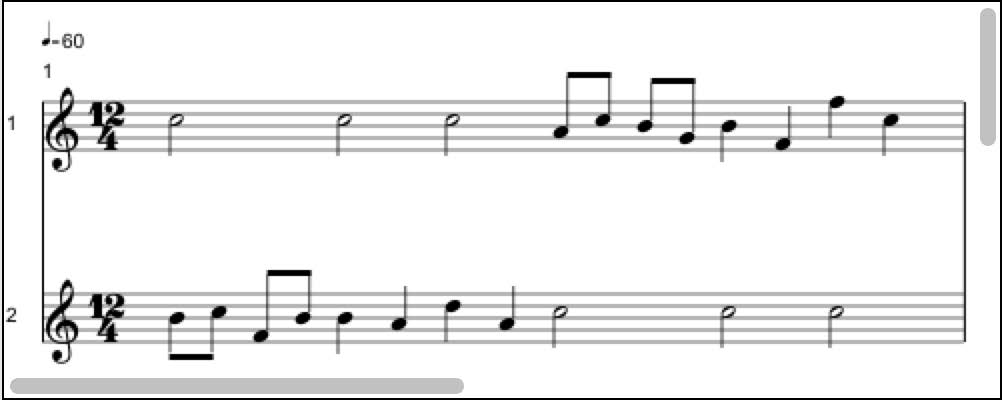
\includegraphics[width=0.9\textwidth]{Tenor-Paper-6.jpg} 
                \caption{A score with a random melody rendered in MaxScore’s default layout.
        \label{fig:Tenor-Paper-6}}
    \end{minipage}\hfill
    \begin{minipage}{0.45\textwidth}
        \centering
        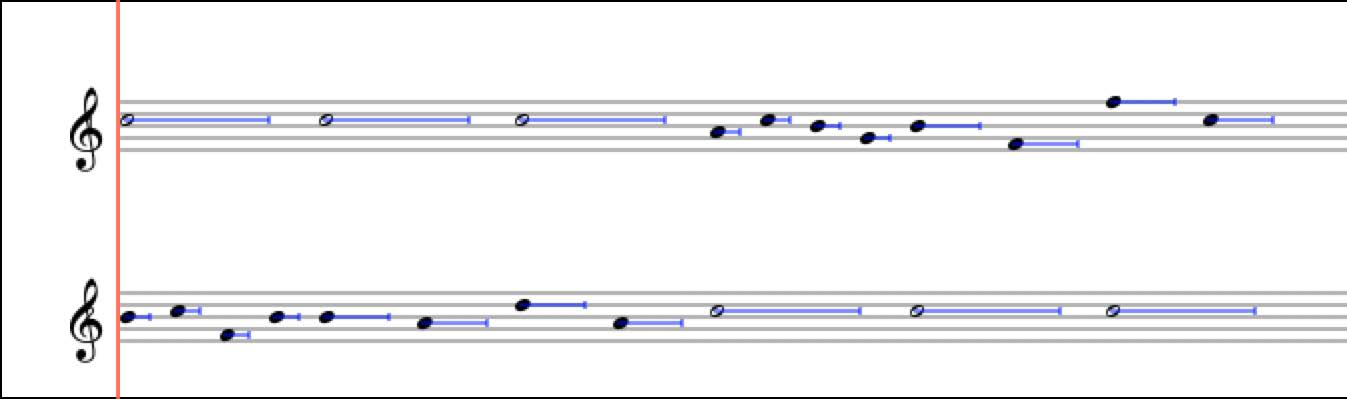
\includegraphics[width=1\textwidth]{Tenor-Paper-7.jpg} 
       	\caption{Same score after applying proportional notation. The default hold times indicated by the blue line is set to 80\% of the event’s nominal duration.
\label{fig:Tenor-Paper-7}}
    \end{minipage}
\end{figure*}

\section{Maxscore}
As mentioned in section~\ref{sec:foundations}., MaxScore possesses a fair amount of flexibility in terms of rendering to a wide array of targets. The JavaScript object render2Browser.js was created to facilitate the communication between the MaxScore object and the hfmt.drawsocket abstraction. The js object was designed with MNMP in mind. Such performances pose enormous difficulties when distributing large scores with dozens of staves. In performances with Quintet.net, scores containing just a few staves were split into instructions to be reassembled by individual instances of the MaxScore object and rendered locally by the Clients. But doing the same with dozen of instances (potentially destabilizing the environment and introducing unwanted latency), we resorted to a different strategy by implementing the concept of multi-client rendering, treating the ensemble of clients like one single canvas. In Maxscore, nearly every rendering message contains indexes referring to the notation object it represents  (Figure~\ref{fig:maxscore-mesages}). Thanks to those indexes, render2Browser.js is capable of dynamically reroute a rendering message to targets set by the staffgroups attribute. This attribute can have the following values: score, parts or a list containing either indexes (for individual staves), two indexes joined by hyphens (for a staff range) or any number of indexes joined by plusses (for arbitrary collections of staves) such as in this example: staffgroups 0 1-2 2 0+3.

In addition to splitting and routing messages, the object is also capable of respacing staves so that resulting layout looks acceptable. It does so by querying the MaxScore object during rendering to obtain crucial information about staff spacing and using this information to apply offsets to the y values of each message to be rendered.

\begin{figure}[h]
\centering
\begin{lstlisting}[ mathescape,
						columns=fullflexible,
						basicstyle=\oscfontsize\fontfamily{lmvtt}\selectfont,
						breaklines=true,
						 frame=single ]
tempoqtrequals 20. 21. 0.5 Measure 0. ...
tr 22. 75.959999 0.5 Staff 0. 0. staffnumber1 0. 63. 0.5 Staff 0. 0. timesig4 43. 57. 0.5 Staff 0. 0.
...
StaffLine 0. 0. 4. 0.5 20. 75. 300.660797 75. false
...
frgb 0 0 0
noteheadblack 83.620689 57. 0.5 Note 0. 0. 0. 0.
frgb 0 0 0
no_accidental 75.555557 57. 0.5 Note 0. 0. 0. 0.
frgb 0 0 0
stem 76.620689 79. 0.5 Note 0. 0. 0. 0. STEM_DOWN
RenderMessage staff 0 0 166. 13. 0.5 
rendered Picster-Element[5] 175.3ocUOsnBBCCCzOk6dAg[...]
\end{lstlisting}

\caption{A sample of rendering messages generated by the MaxScore object. 
\label{fig:maxscore-mesages}}
\end{figure}

Figure \ref{fig:maxscore-mesages} shows a sample of rendering messages generated by the MaxScore object. Note that nearly every message is accompanied by indexes (in red) referring to the notation object they represent. The y coordinates (blue numbers) are remapped according to the current staffgroups setting. The RenderMessage message contains a gzip’ed JSON object which in turn codes for a graphical score element such as a line, a rectangle, an arc or an image.

render2Browser.js is also capable of animating any number of cursors moving across set of measures and staves (see TENOR 2018 paper).

\begin{figure*}[h]
    \centering
    \begin{minipage}{1.\textwidth}
        \centering
        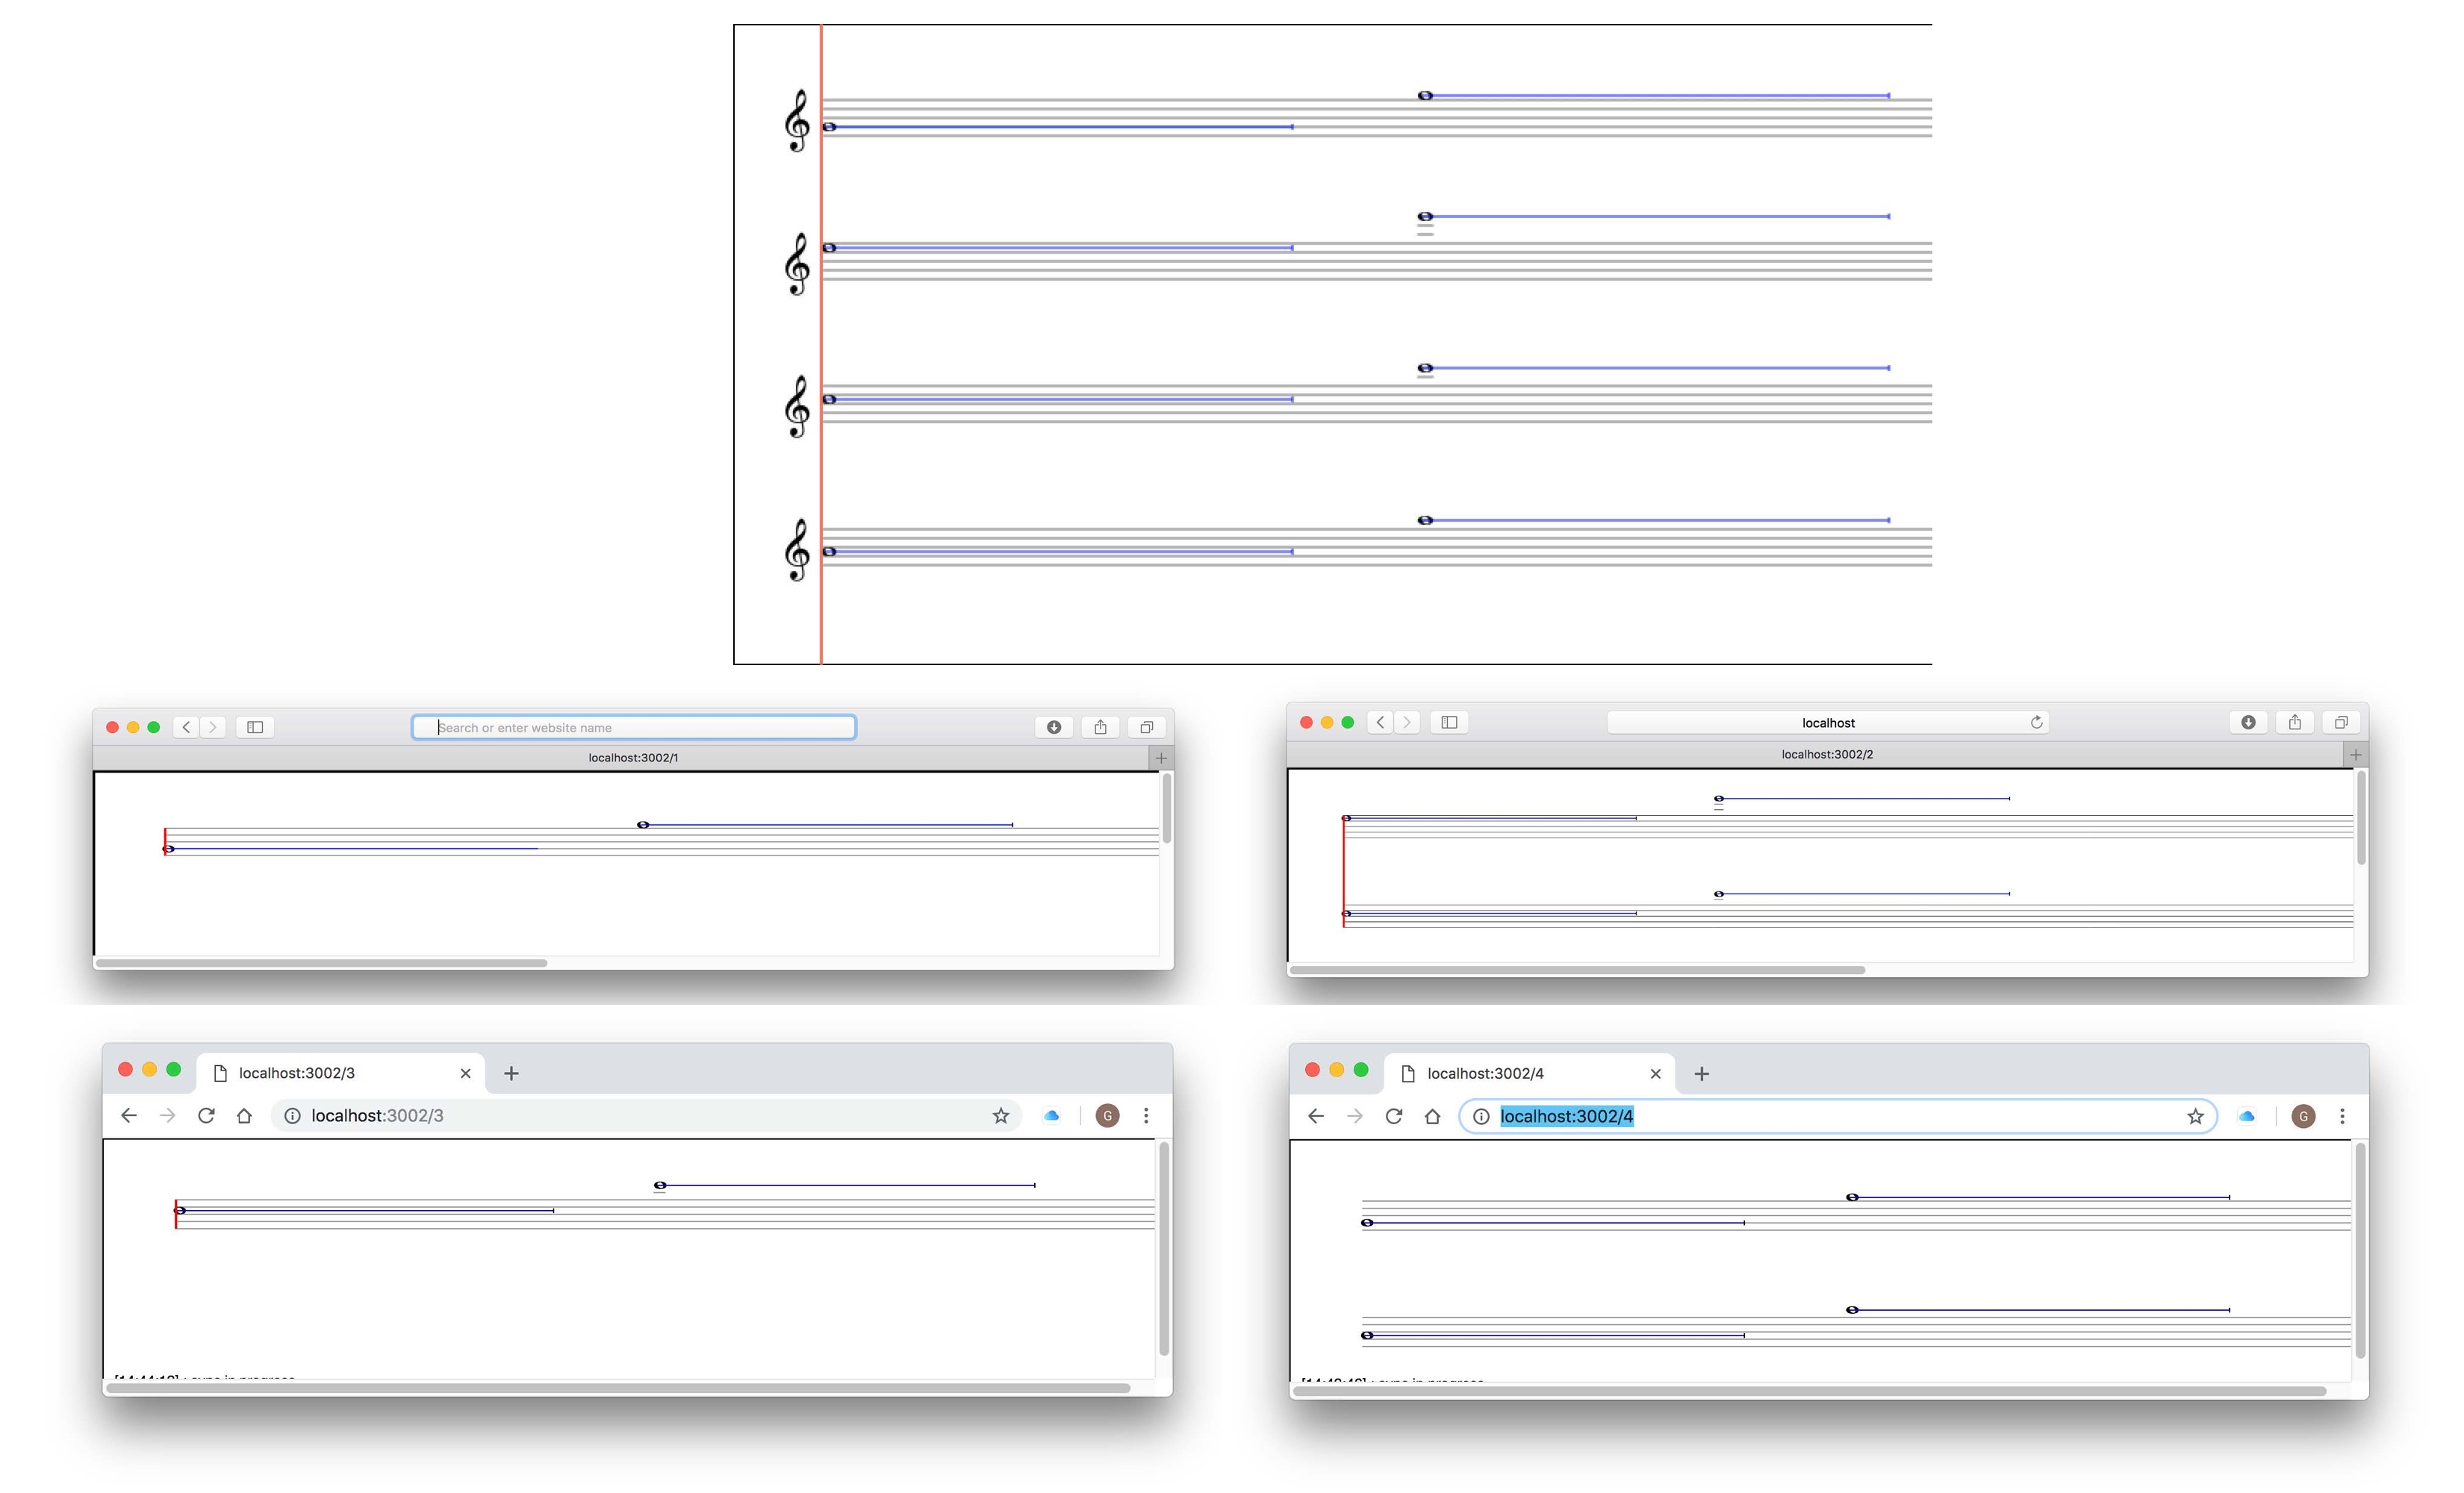
\includegraphics[width=1\textwidth]{Tenor-Paper.png} 
       	\caption{A MaxScore score with 4 staves (top) rendered dynamically in four browser windows (center and bottom). The staves are split and grouped by render2Browser.js according to the following staffgroup settings: 0 1-2 2 0+3.
\label{fig:Tenor-Paper}}
    \end{minipage}
\end{figure*}


To scroll the entire score horizontally, we created another JavaScript object called maxscore.proportionalNotation.js. It toggles between MaxScore’s default score layout and its proportional representation by hiding rests, stems, beams and naturals and indicating the duration of a note by a line extending from a note. The length of a measure is calculated by obtaining its tempo and time signature values and taking a setTimeUnit attribute into consideration. The durational scaling base value of 0.385 has proven to be optimal for spatially representing the delta time between events. The start message will cause a playhead to appear at the position given by the scoreLeftMargin attribute and instruct the browser to scroll the score. We are planning to also support scores created for the Decibel ScorePlayer in the future. 



%describe use of hfmt.drawsocket via Maxscore translation script.




\section{Case study}

A new  piece (Raindrops Keep Falling) by Georg Hajdu was premiered at the December 2018 WOCMAT conference in Hsinchu, Taiwan. This composition for clarinet, cello and percussion with multimedia consists of a transition between various rain samples and a late-1960’s hit called Raindrops Keep Fallin' On My Head mediated by a Max Pluggo effect called Raindrops. It’s also a tongue-in-cheek reference to the usual end-of-year weather pattern in Taiwan. The piece features 12 different versions of the song found on the Internet. The HfMT graduate student and research assistant James Cheung arranged the songs in such manner that they all share the same tempo structure and key signature, allowing the seamless navigation between those versions. James also created an arrangement of the song for the aforementioned instrumentation to be performed simultaneously with the recording, which was further subject to processing. First, parts of the score were “whited out” by a probabilistic process so that more and more events were allowed to appear paralleling a similar process applied to the audio tracks. The whiting-out was achieved by a JavaScript object called maxscore.whiteout.js capable of applying a “whiteout” gradient to a given section (the name was inspired by Cat Hope’s piece The Great White). Second, the score was turned into proportional notation, transmitted to the iPads of the performers via hfmt.drawsocket and scrolled in synch with the audio. The system held up to its promise as a computer-based conducting system. The scrolling was fluid and the musicians stayed in tempo despite the tempo fluctuations in the audio track. 

\begin{figure*}[h]
    \centering
    \begin{minipage}{0.6\textwidth}
        \centering
        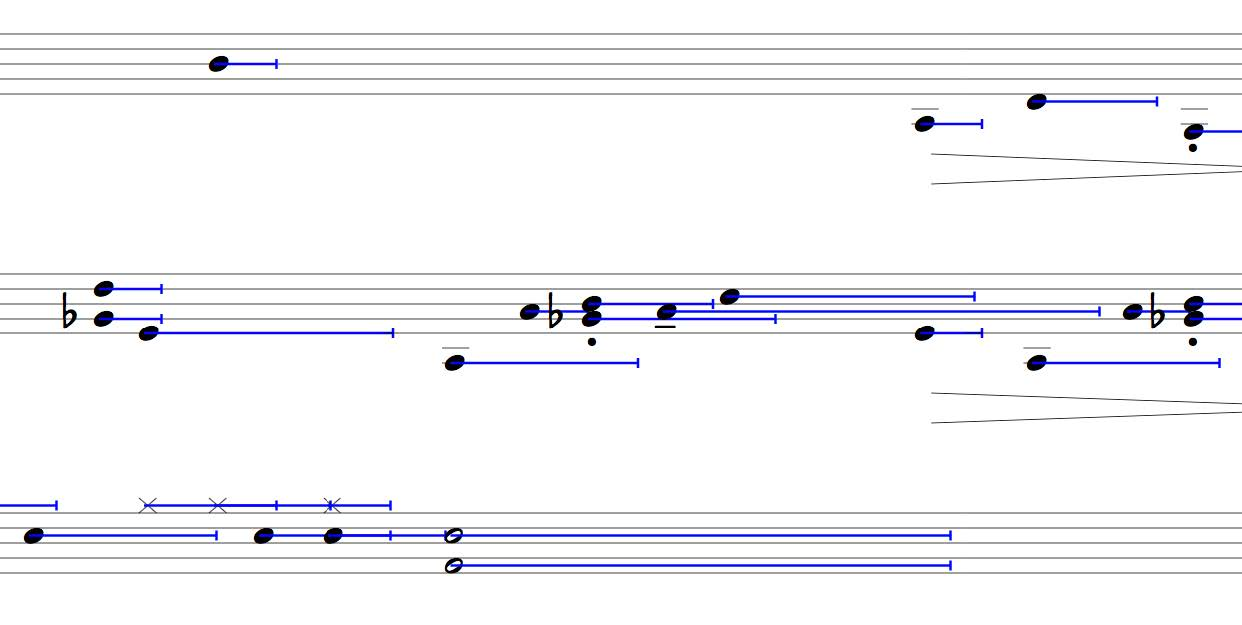
\includegraphics[width=1\textwidth]{Tenor-Paper-8.jpg} 
       	\caption{Excerpt from Raindrops Keep Falling (2018) for clarinet, cello, drum set and multimedia.
\label{fig:Tenor-Paper-8}}
    \end{minipage}
\end{figure*}





\section{Future Work}

\drawsocket currently still considered ``in development'', that said, the system has already been used in several live performances, and appears to be fairly robust.
As we prepare for the large-scale extension of the system to the St. Pauli Elbtunnel~\cite{elbtunnel19} we will have a good opportunity to fully stress-test the system.

One potential issue that we imagine could arise is with the caching system. 
Currently the caching routine is processed within the callback function that gets called when a new dictionary arrives from Max.
On receiving a new dictionary, the server routes the data, sending packets to the appropriate clients, and then sends the packets to the cache system which unions the data with any nodes with a matching \textit{id} (or \textit{selector} in the case of CSS).
There is a question about the scalability of this approach. 

Node.js, like vanilla JS, uses an ``event driven'', ``single threaded event loop model'', which uses a queue of event callbacks which need to be processed asynchronously.
However, it is possible to block the event loop\cite{node-eventloop} within a callback function, should the execution take too long.
In particular, the JSON.parse and JSON.stringify operations are potentially expensive, with a complexity of $O(n)$; so, depending on the size of the incoming dictionary, this could significantly slow down the response of the server.
In our testing so far, we have already noticed some issues with processing very large dictionaries arriving from Max, but we need to investigate further.
It is possible that since the data is broadcasted before being sent to the caching system, that the blocking of the event loop will be less noticeable on the client-side, however, the responsiveness of the server will be reduced and this will likely effect the clock-synchronization routine, and could also in extreme cases result in a buildup of events to process in queue.
To address this issue, we might look into storing the URL states in a separate database, which runs as a separate process.


\begin{acknowledgments}
The authors would like to thank Jacob Sello for his detailed testing the system which pushed the development of many new features and design considerations. We would also like to acknowledge the Federal Ministry of Education and Research in Germany (BMBF), for their support of this research through the Innovative Hochschule: Stage\_2.0 initiative.
\end{acknowledgments} 

%%%%%%%%%%%%%%%%%%%%%%%%%%%%%%%%%%%%%%%%%%%%%%%%%%%%%%%%%%%%%%%%%%%%%%%%%%%%%
%bibliography here
\balance
\bibliography{symbolist}
\end{document}




